% Bubble grid
\subsection{Google Trends}

We have some data in a csv giving Google search trend popularity by month for computer scientist \link{https://en.wikipedia.org/wiki/Grace_Hopper}{Grace Hopper} and Nobel Prize-winning economist \link{https://en.wikipedia.org/wiki/Elinor_Ostrom}{Elinor Ostrom}. We'll try visualizing the trends with a few heatmaps.

First, let's import the data. We can even look at the data in a table with matplotlib if for some sick reason you want to use matplotlib for such a task.
\pyfile{mpl-table.py}


\begin{center}
    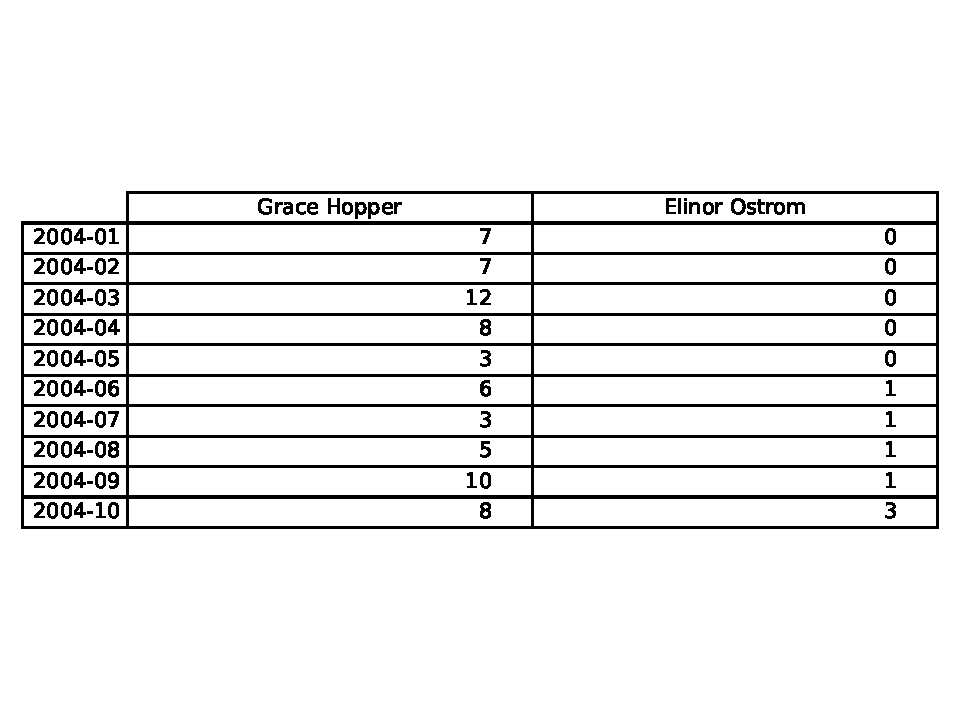
\includegraphics[width = .8\textwidth]{figures/poetryplots/mpl-table.pdf}
\end{center}

A table is capital-B Boring. A \code{df.plot()} line chart would display these trends very well, but let's move on to making a heatmap. Here we'd have just two lines, but imagine we had several more columns in our dataset. The line chart would become a spaghetti chart. Heatmaps can be useful in avoiding this by giving each data series its own lane. Take this as a toy example of an application that helps when you have that additional clutter. 

\begin{center}
    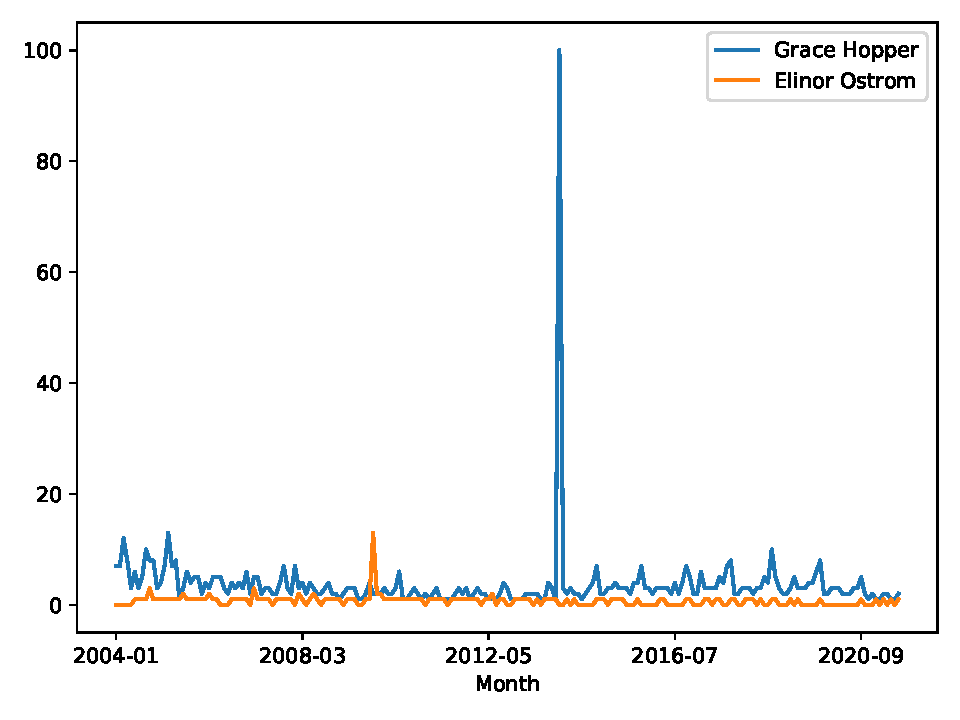
\includegraphics[width = .8\textwidth]{figures/poetryplots/df-plot.pdf}
\end{center}

Matplotlib offers the \code{imshow()} axes method especially for this purpose. Later, we'll create our own heatmap simply by adding our own artist objects to the plot. 

\subsubsection{Using \code{imshow()}}

First can call \code{imshow()} with our transposed dataframe to get a sense of what the method does. The transpose is done so that the time (the rows of the DataFrame) will be on the $x$-axis. The \code{aspect} argument essentially makes the chart taller. With \code{aspect} set to 20, each cell is 20 times taller than it is wide. Finally, I change the colormap with \code{cmap = 'Oranges'} to create a monochromatic map where a darker orange is a higher search volume. 

\pyfile{heat-basic.py}

\begin{center}
    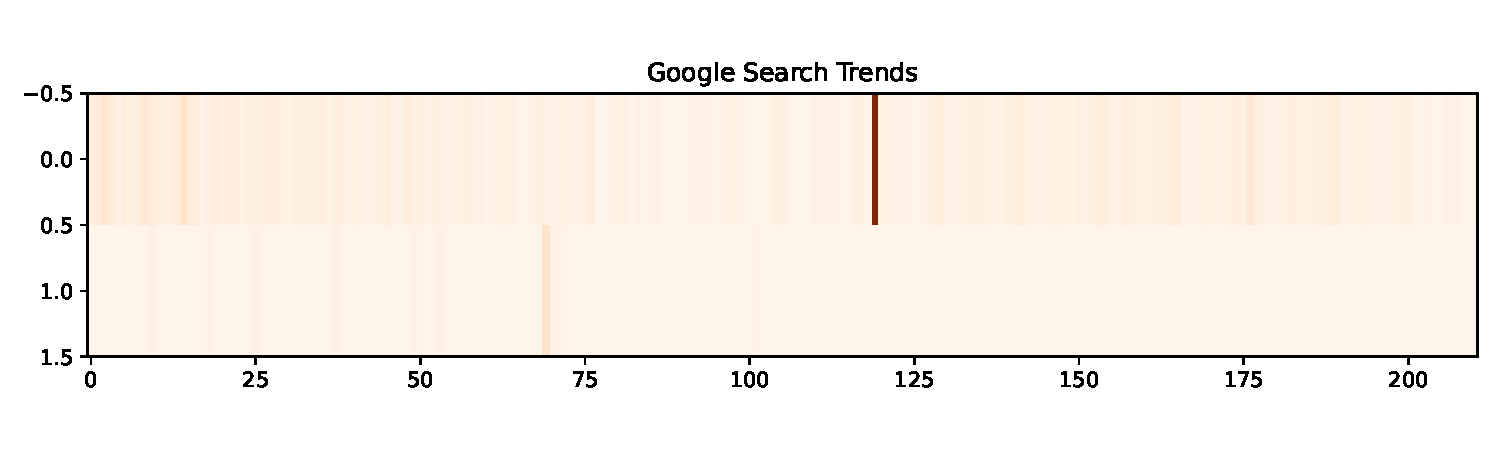
\includegraphics[width = .8\textwidth]{figures/poetryplots/heat-basic.pdf}
\end{center}

One obvious problem with this is we have no useful labels or ticks, unlike what we'd get for free with a simple \code{df.plot()} call. This will be remedied with the ticks customizations we learned about in Section \ref{sec:ticks}. Another problem is that our data is not well behaved. The trends are washed out because of an outlier. In December 2013, Grace Hopper was featured in the Google Doodle, driving a lot of searches. All other months pale in comparison. By default, \code{imshow} uses a linear scaling mapping where the lowest value is at the bottom of the colormap and the highest value is at the top of the colormap. As a result almost, all observations are toward the bottom of the colormap. One could transform the data directly or one could change the behavior of \code{imshow()}. We can transform the data with the \code{norm} argument or manually set the top and bottom values of the colormap with \code{vmin} and \code{vmax}. 

First we use \code{mpl.colors.LogNorm()} to take a log transform of the data before normalizing. We also thin the $x$-axis ticks manually (instead of using a Formatter) and then relabel the ticks manually. 

\pyfile{heat-log.py}

\begin{center}
    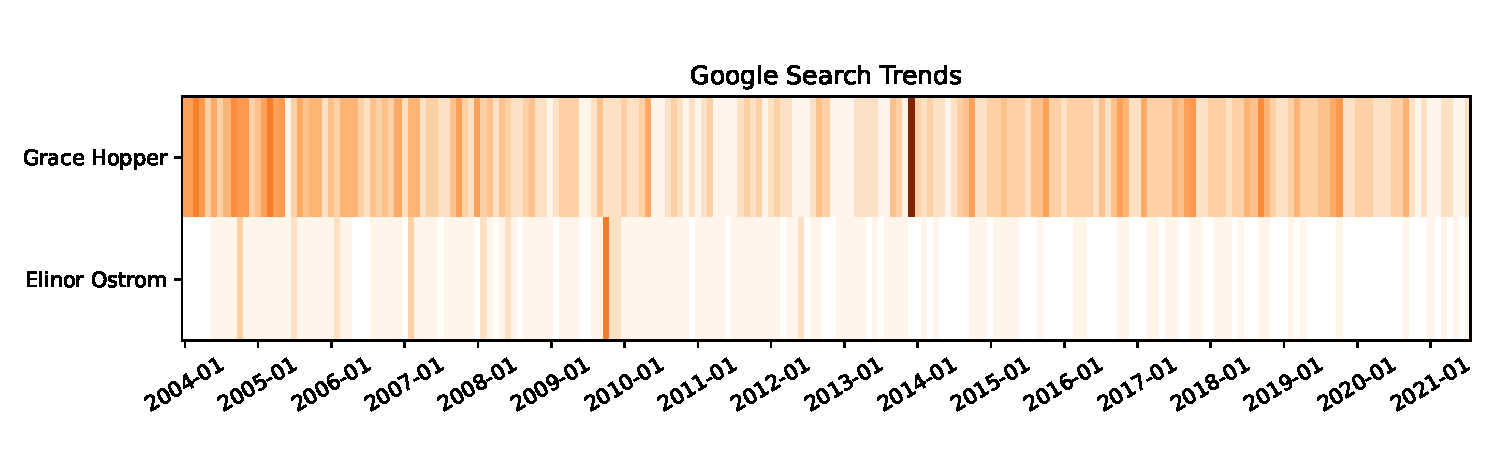
\includegraphics[width = .8\textwidth]{figures/poetryplots/heat-log.pdf}
\end{center}

The data transformation helps the trends seen in the original line chart pop more prominently. Elinor Ostrom's search interest has remained steady but for a spike in 2009 when she was awarded the Nobel Prize in Economics, along with Oliver Williamson. The surge in search interest for Grace Hopper because of the 2013 Google Doodle remains noticeable, but the yearly spikes in interest around the Grace Hopper conference (usually held around the beginning of October) are more noticeable. Perhaps you find the transformation makes the heatmap too noisy. We can keep the quiet of the original linearly-scaled heatmap, but make but make spikes in interest more visible by lowering the point at which the color gradient maxes out. Below we do this by lowering \code{vmax}. By default, \code{vmax} uses the maximum data value (100 in our case). Setting \code{vmax = 50} means values from 50 to 100 are not differentiated by color in the heatmap. We'll also add a colorbar.

\pyfile{heat-cbar.py}

\begin{center}
    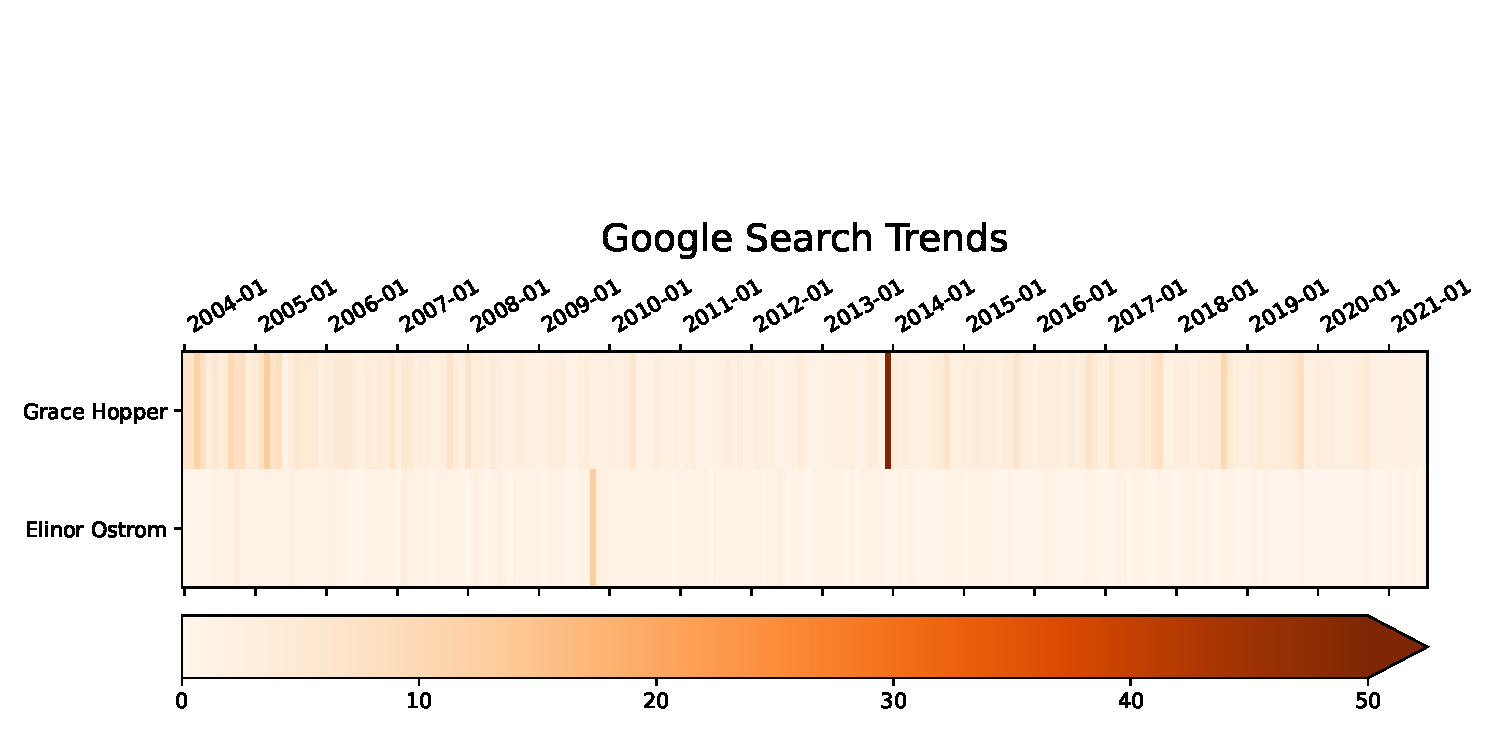
\includegraphics[width = .8\textwidth]{figures/poetryplots/heat-cbar.pdf}
\end{center}


\subsection{NHL Regular Season Records}

WIP. Below is a kind of a heatmap. 

\pyfile{hockey-heat.py}

\begin{center}
    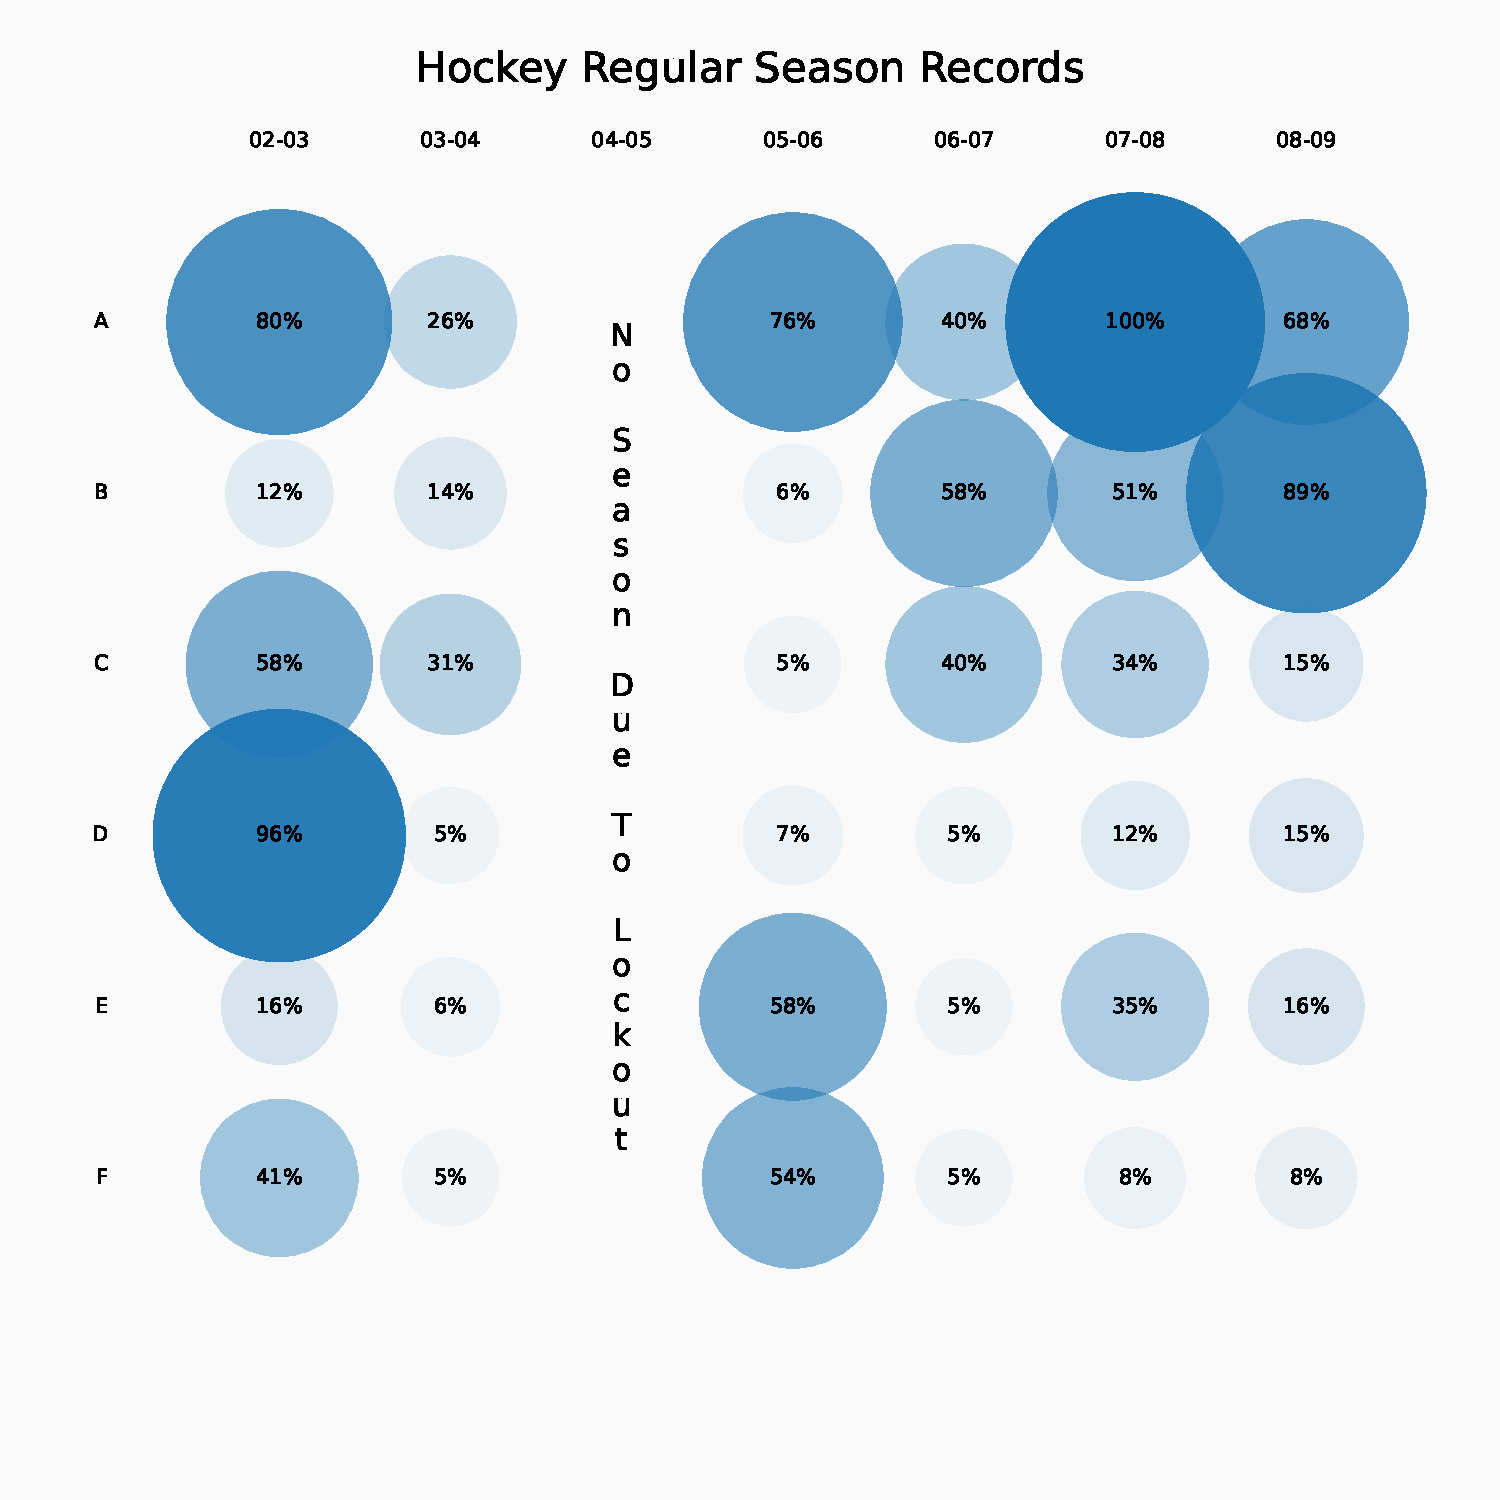
\includegraphics[width = .7\textwidth]{figures/poetryplots/hockey-heat.pdf}
\end{center}